\documentclass[letterpaper,11pt]{article}
\usepackage{graphicx}
\usepackage{listings}
\usepackage[super]{nth}
\usepackage[hyphens]{url}
\usepackage{hyperref}
\usepackage{amsmath}
\usepackage[makeroom]{cancel}
\usepackage[table]{xcolor}
\usepackage{comment}
\usepackage[space]{grffile}
\usepackage{csvsimple}
\usepackage{longtable}


\newcommand*{\srcPath}{../src}%

\lstset{
	basicstyle=\footnotesize,
	breaklines=true,
}

\begin{document}

\begin{titlepage}

\begin{center}

\Huge{Assignment 10}

\Large{CS 532:  Introduction to Web Science}

\Large{Spring 2017}

\Large{Grant Atkins}

\Large Finished on \today

\end{center}

\end{titlepage}

\newpage


% =================================
% First question
% =================================
\section*{1}

\subsection*{Question}

\begin{verbatim}
1.  Using the data from A8:

- Consider each row in the blog-term matrix as a 
1000 dimension vector, corresponding to a blog.  

- From chapter 8, replace numpredict.euclidean() with 
cosine as the distance metric. In other words, you'll 
be computing the cosine between vectors of 1000 dimensions.  

- Use knnestimate() to compute the nearest neighbors for both:

http://f-measure.blogspot.com/
http://ws-dl.blogspot.com/

for k={1,2,5,10,20}.
\end{verbatim}

\clearpage
\subsection*{Answer}


\lstinputlisting[firstline=48,lastline=87,frame=single,caption={Python script with included cosine function and knnestimate},label=lst:q1download,captionpos=b,numbers=left,showspaces=false,showstringspaces=false,basicstyle=\footnotesize]{\srcPath/numpredict.py}

% firstline=48,lastline=87

\begin{table}[htb]
\centering
\begin{tabular}{ | l | l | l | l |}
\hline
\textbf{Source User} & \textbf{Target User} & \textbf{Following Target} & \textbf{Followed By Target} \\
\hline
\end{tabular}
\caption{Format of friendships.csv, where Following fields are booleans}
\label{table:q1csvtable}
\end{table}



\clearpage
 \begin{figure}[h]
 \centering
 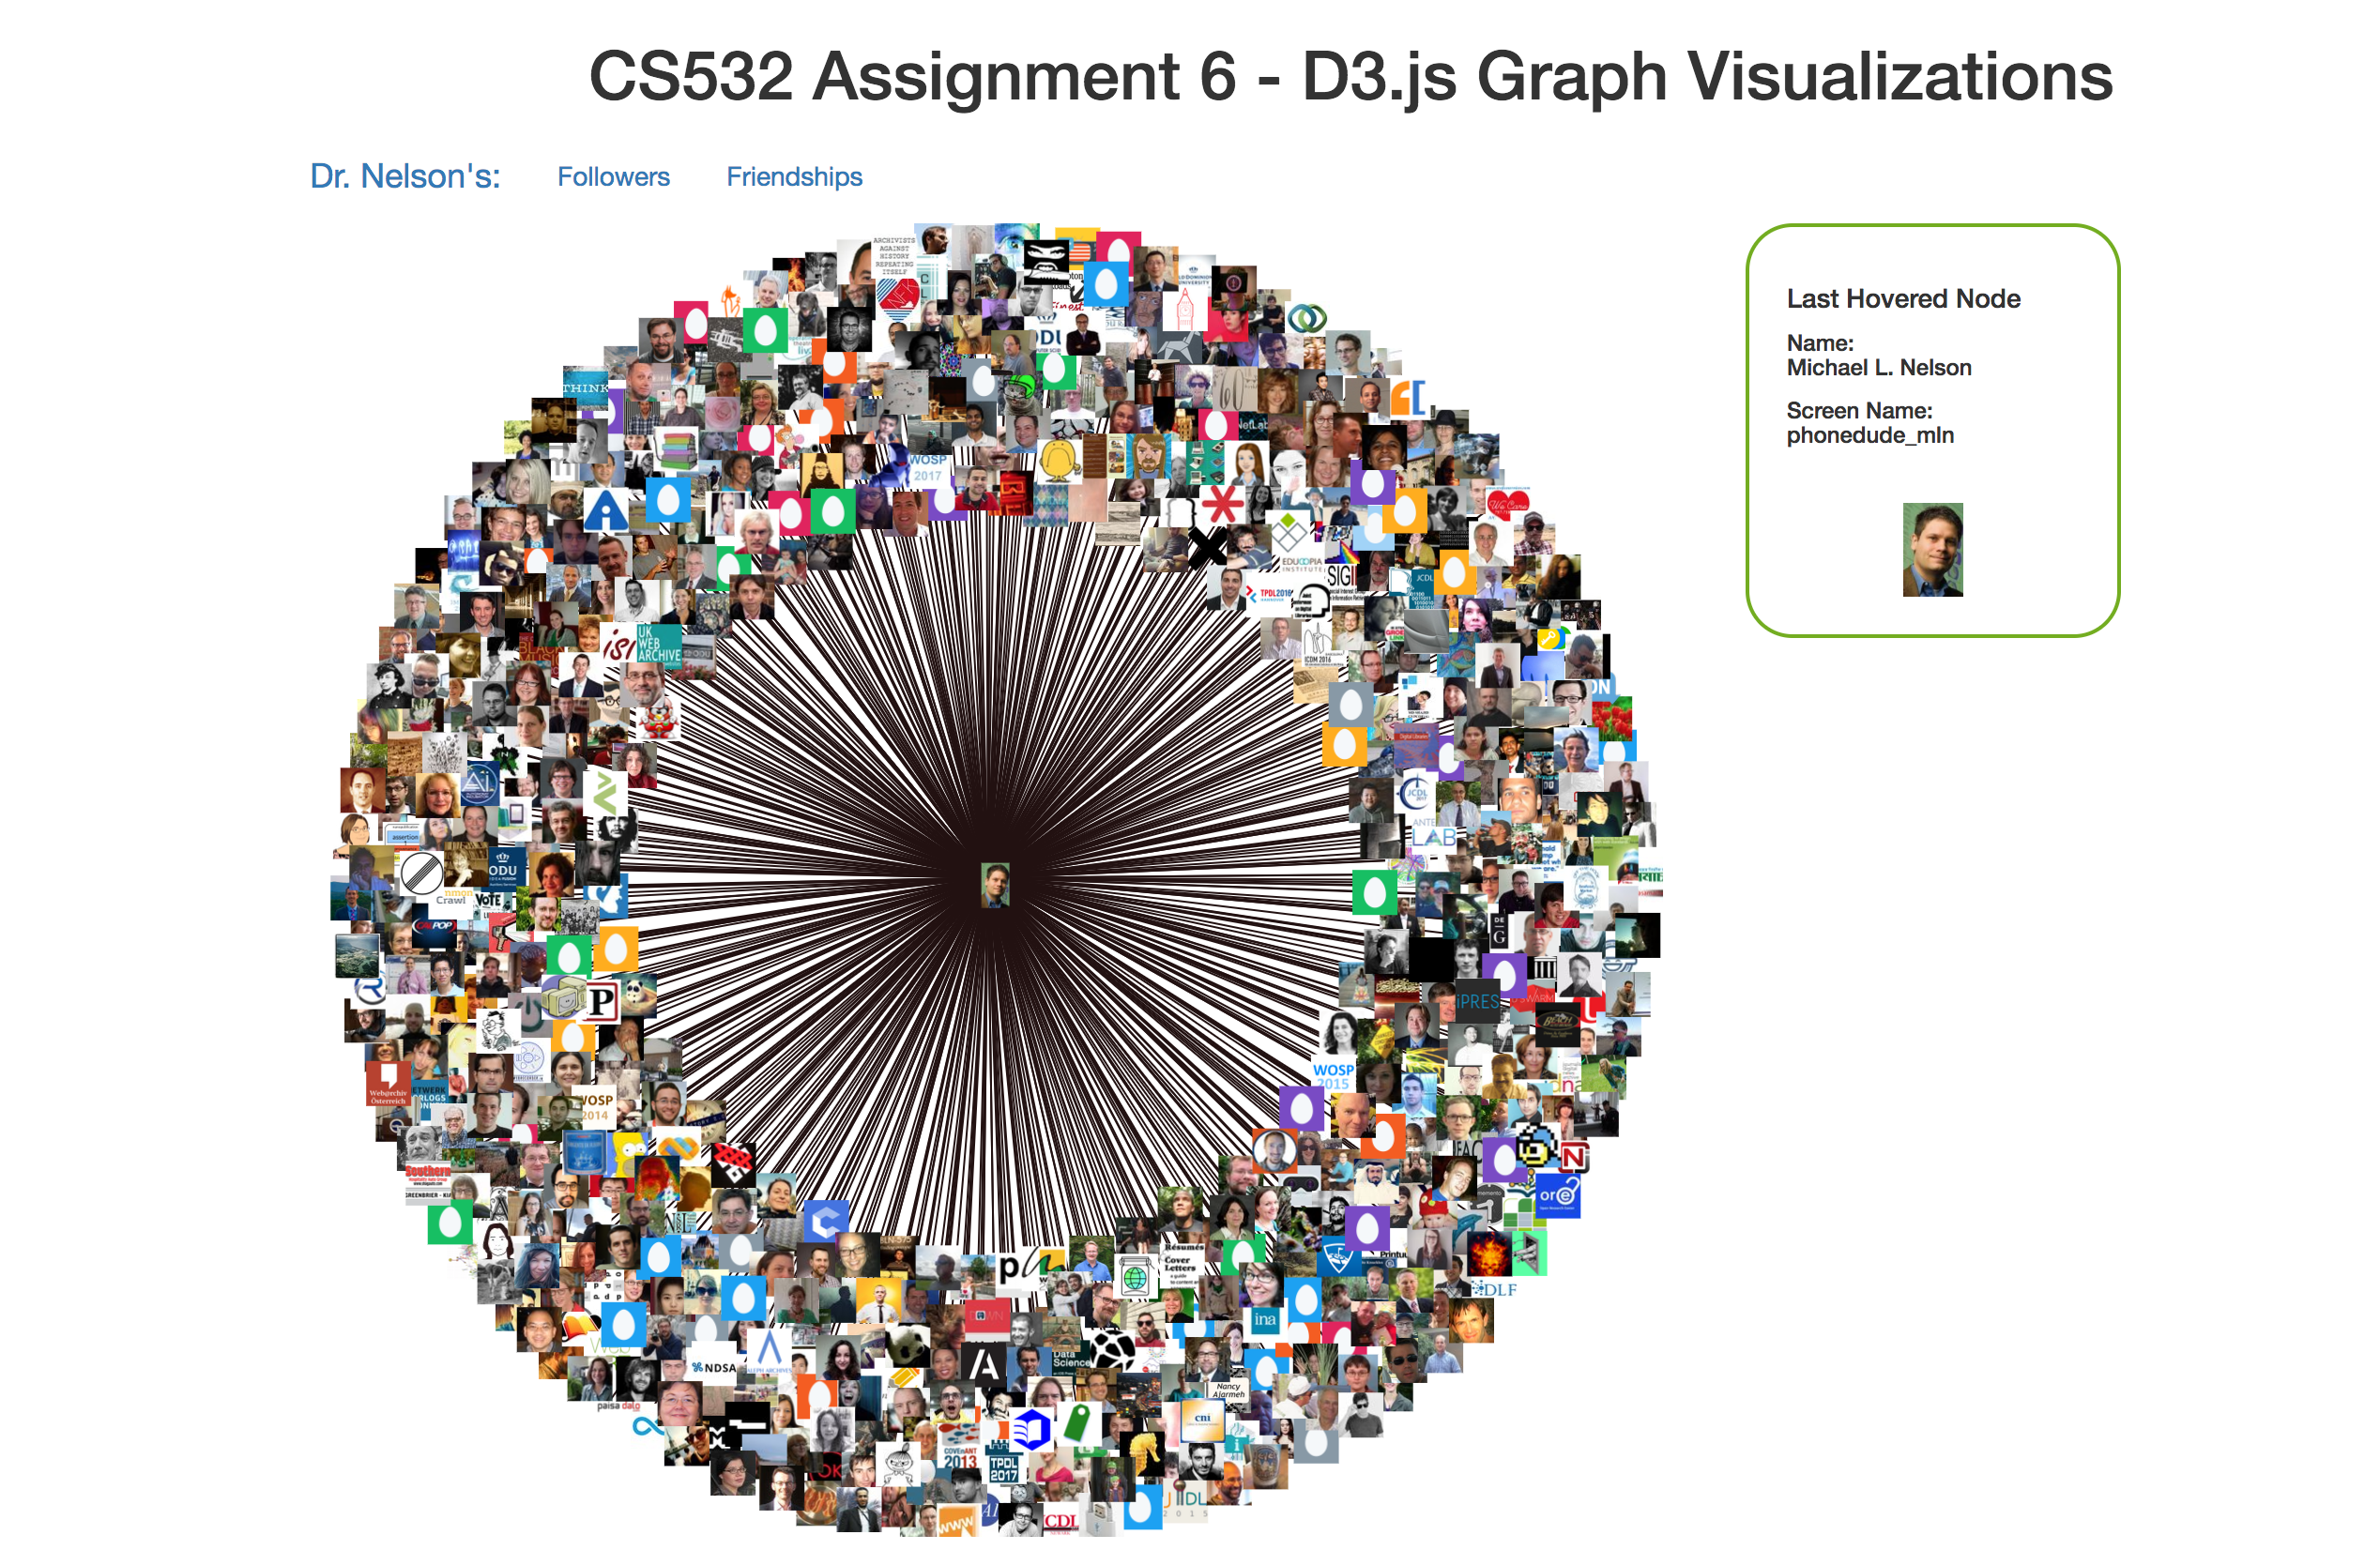
\includegraphics[scale=0.4]{d3followerGraph.png}
 \caption{All of Dr. Nelson's followers in D3 force directed graph}
 \label{fig:q1friendshipgraph}
 \end{figure}


\clearpage

% =================================
% Second question
% =================================

\section*{2}

\subsection*{Question}

\begin{verbatim}
2.  Rerun A9, Q2 but this time using LIBSVM.  If you have 
n categories, you'll have to run it n times.  For example, 
if you're classifying music and have the categories:

metal, electronic, ambient, folk, hip-hop, pop

you'll have to classify things as:

metal / not-metal
electronic / not-electronic
ambient / not-ambient

etc.

Use the 1000 term vectors describing each blog as the features, and
your mannally assigned classifications as the true values.  Use
10-fold cross-validation (as per slide 46, which shows 4-fold
cross-validation) and report the percentage correct for 
each of your categories.
\end{verbatim}

\subsection*{Answer}

After reading many stackoverflow posts on LIBSVM, I decided to use scikit-learn library to solve this question \cite{stack1}. 


% \begin{figure}[h]
% \centering
% 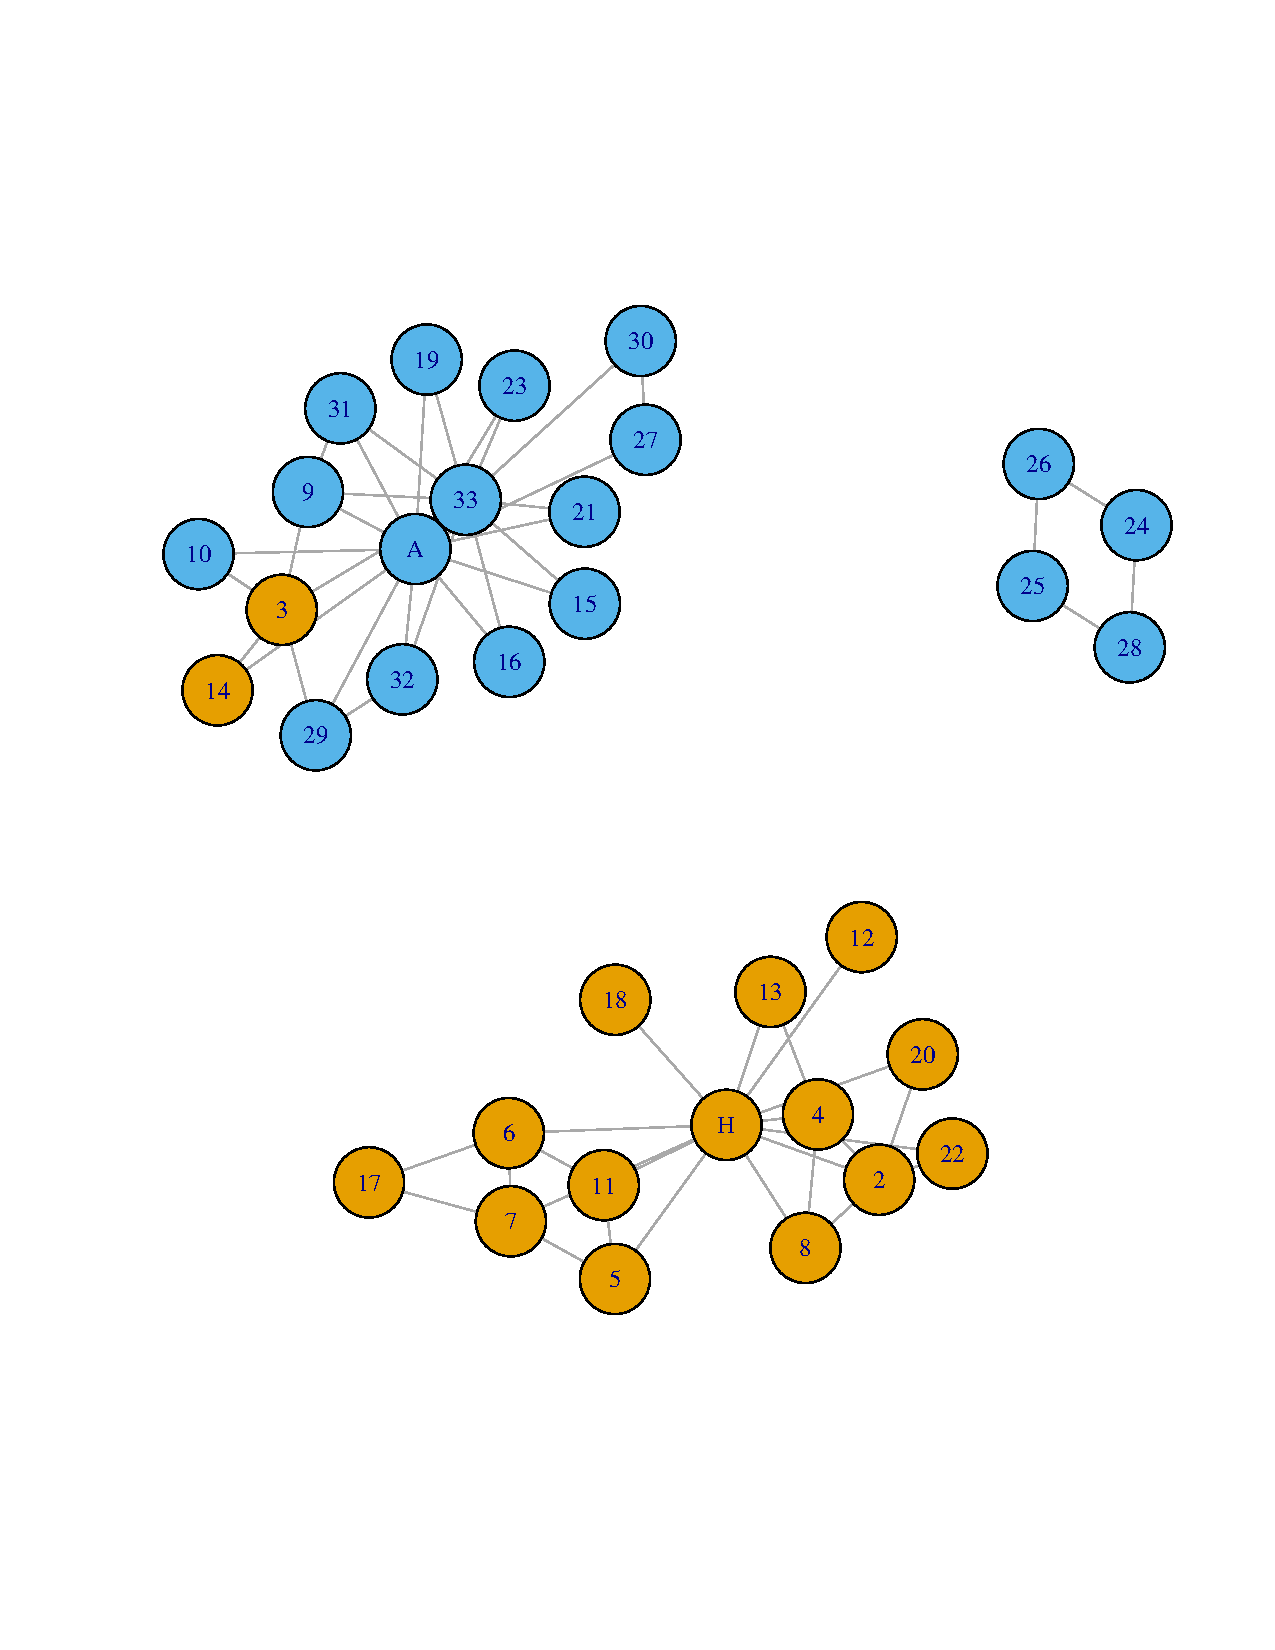
\includegraphics[scale=0.6]{predictedSplit3.pdf}
% \caption{Group split of 3 with Girvan-Newman algorithm from karateClub.R}
% \label{fig:split3}
% \end{figure}

\clearpage

% =================================
% 3rd question
% =================================

\section*{3}

\subsection*{Question}

\begin{verbatim}
(3 points extra credit)

3. Re-download the 1000 TimeMaps from A2, Q2.  Create a graph where
the x-axis represents the 1000 TimeMaps.  If a TimeMap has "shrunk",
it will have a negative value below the x-axis corresponding to the
size difference between the two TimeMaps.  If it has stayed the
same, it will have a "0" value.  If it has grown, the value will be 
positive and correspond to the increase in size between the two
TimeMaps.

As always, upload all the TimeMap data.  If the A2 github has the 
original TimeMaps, then you can just point to where they are in 
the report.
\end{verbatim}

\subsection*{Answer}

\begin{center}
\Huge{NOT ATTEMPTED}
\end{center}

% \begin{figure}[h]
% \centering
% 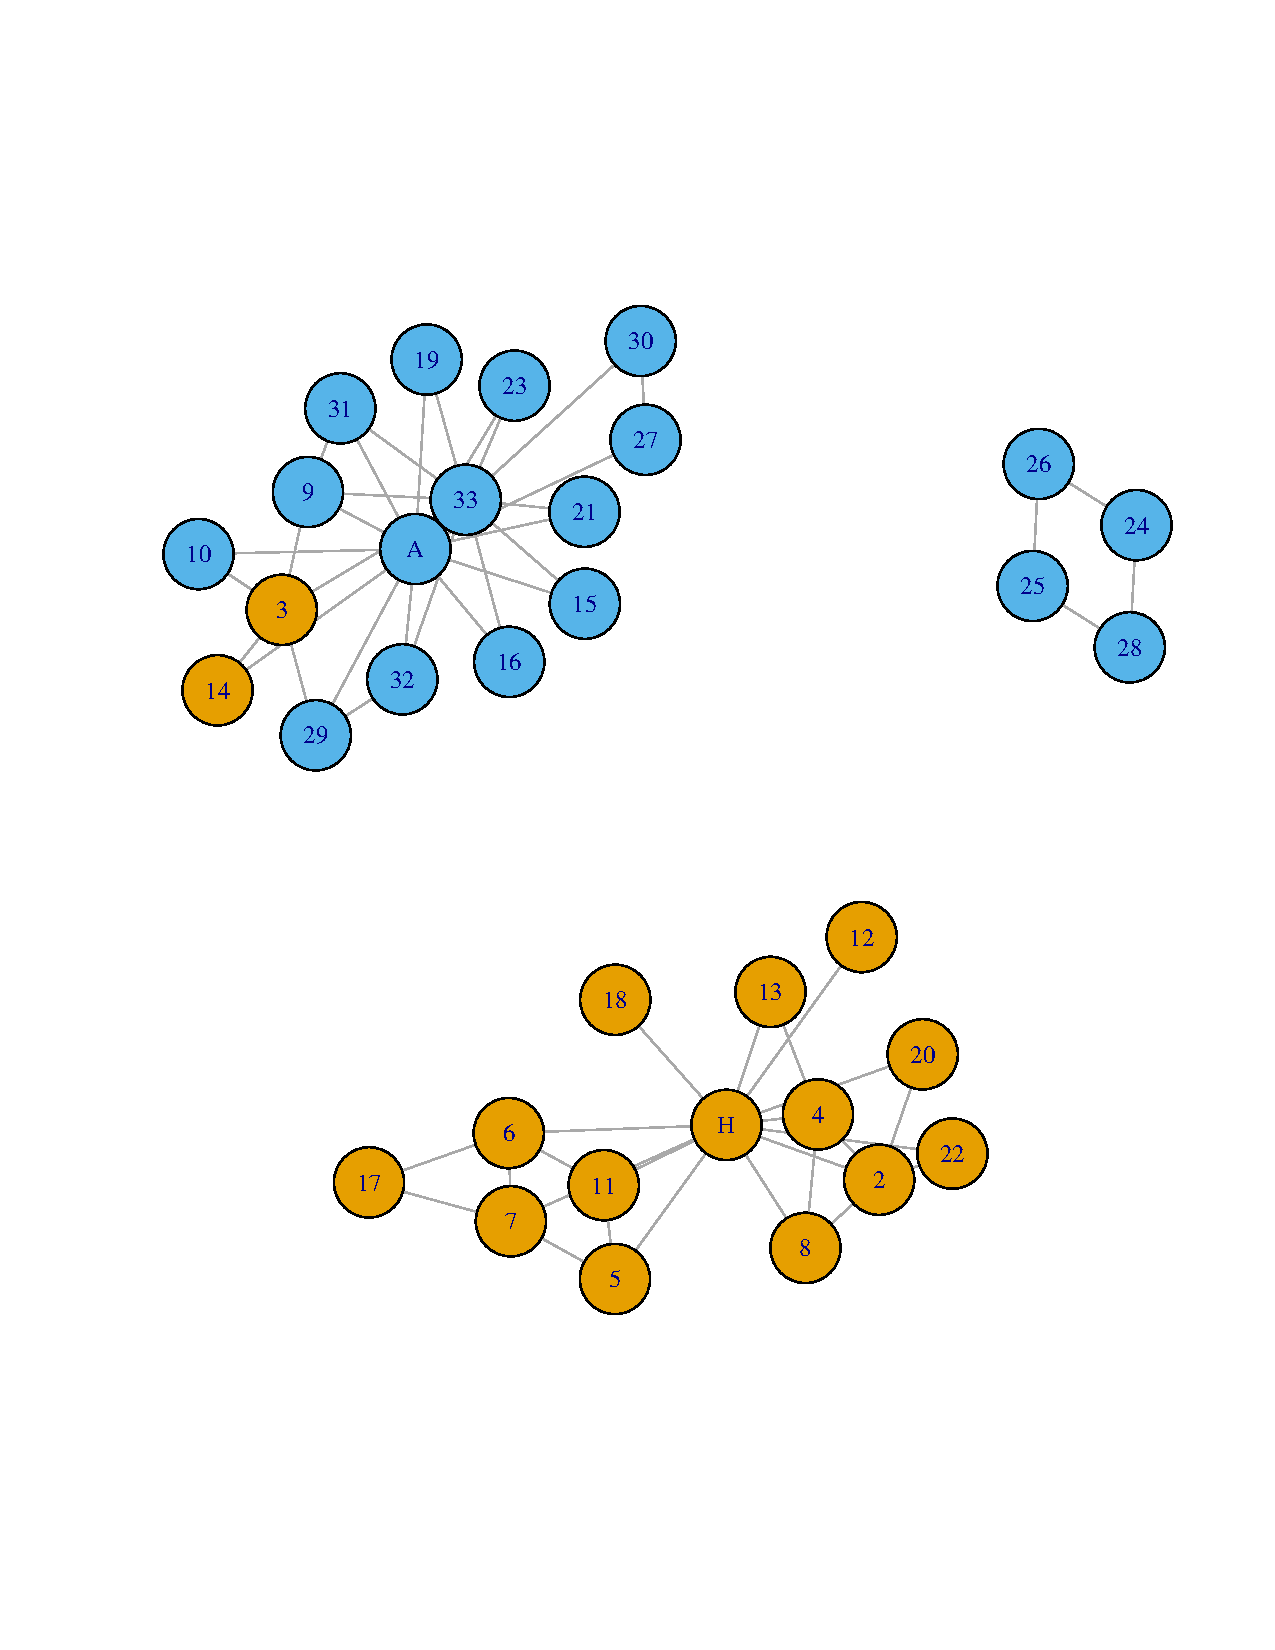
\includegraphics[scale=0.6]{predictedSplit3.pdf}
% \caption{Group split of 3 with Girvan-Newman algorithm from karateClub.R}
% \label{fig:split3}
% \end{figure}


% =================================
% 4th question
% =================================

\section*{4}

\subsection*{Question}

\begin{verbatim}
(3 points extra credit)

4.  Repeat A3, Q1.  Compare the resulting text from February to 
the text you have now.  Do all 1000 URIs still return a "200 OK" 
as their final response (i.e., at the end of possible redirects)?

Create two graphs similar to that described in Q3, except this 
time the y-axis corresponds to difference in bytes (and not difference
in TimeMap magnitudes).  For the first graph, use the difference
in the raw (unprocessed) results.  For the second graph, use the 
difference in the processed (as per A3, Q1) results.

Of the URIs that still terminate in a "200 OK" response, pick the
top 3 most changed (processed) pairs of pages and use the Unix
"diff" command to explore the differences in the version pairs.
\end{verbatim}

\subsection*{Answer}

\begin{center}
\Huge{NOT ATTEMPTED}
\end{center}

% \begin{figure}[h]
% \centering
% 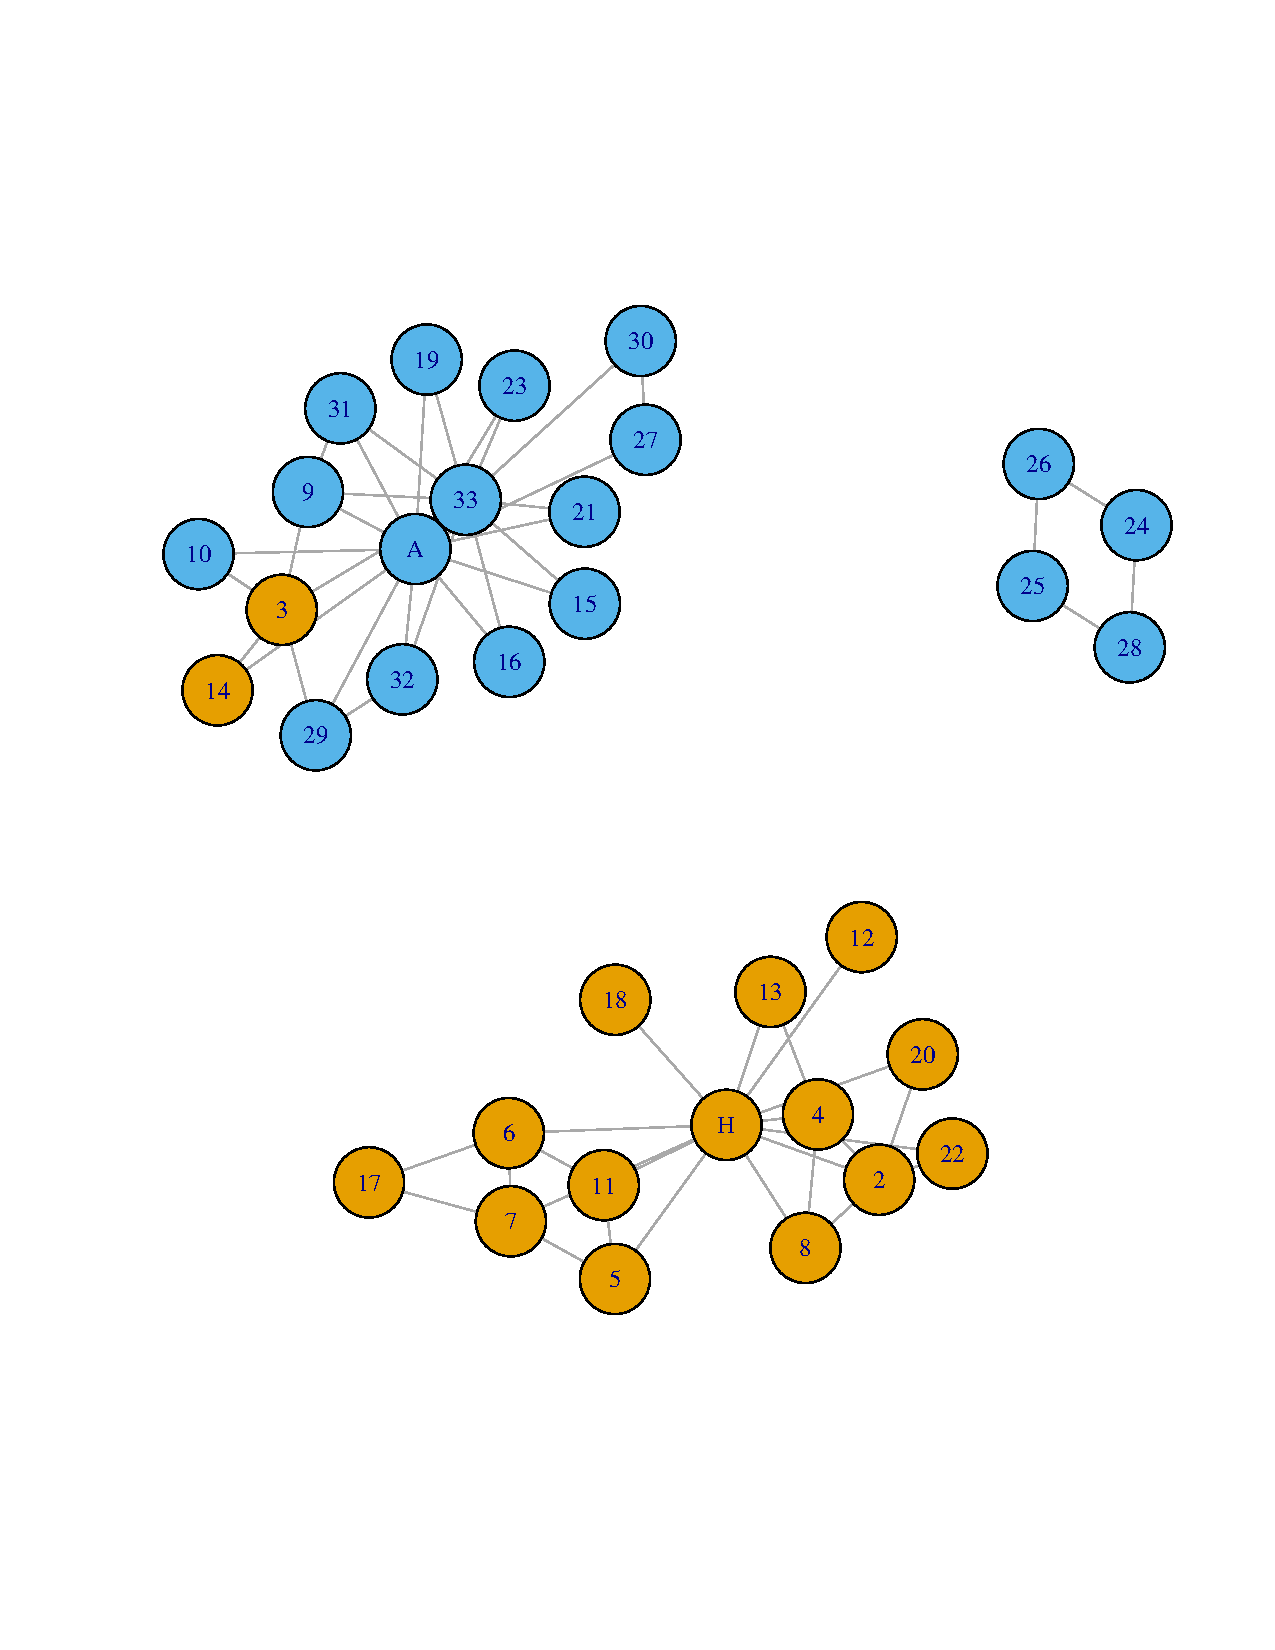
\includegraphics[scale=0.6]{predictedSplit3.pdf}
% \caption{Group split of 3 with Girvan-Newman algorithm from karateClub.R}
% \label{fig:split3}
% \end{figure}

\clearpage


\clearpage


% =================================
% Bibliography
% =================================

\begin{thebibliography}{9}
\bibitem{github}
Atkins, Grant. ``CS532 Assignment 10 Repository'' Github. N.p., 23 March 2017. Web. 23 March 2017.\url{https://github.com/grantat/cs532-s17/tree/master/assignments/A10}.
\bibitem{collectiveIntell}
Segaran, Toby. ``Programming Collective Intelligence''. O' Reilly, 2007. Web. 6 April 2017. \url{http://shop.oreilly.com/product/9780596529321.do}.
\bibitem{stack1}
``How to setup LIBSVM for Python''. n.p., n.d. Web. 1 May 2017. \url{http://stackoverflow.com/questions/15755130/how-to-setup-libsvm-for-python}
\end{thebibliography}

\end{document}